\documentclass[aspectratio=169]{beamer}
%\documentclass[aspectratio=43]{beamer}

\usepackage{graphicx}  % Required for including images
\usepackage{natbib}
\usepackage{booktabs} % Top and bottom rules for tables
\usepackage{amssymb,amsthm,amsmath}
\usepackage{exscale}
\usepackage{natbib}
\usepackage{tikz}
\usepackage{listings}
\usepackage{color}
\usepackage{animate}
\usepackage{bm}
\usepackage{etoolbox}

% Setup TikZ
\usepackage{tikz}
\usetikzlibrary{arrows}
\tikzstyle{block}=[draw opacity=0.7,line width=1.4cm]
% Setup hyperref
\usepackage{hyperref}
\hypersetup{colorlinks=true}
\hypersetup{citecolor=porange}
\hypersetup{urlcolor=porange!80!}
\hypersetup{linkcolor=porange}

\newtheorem{proposition}{Proposition}
\newtheorem{remark}{Remark}
\newtheorem{principle}{Principle}

%% Writing quarters
\newcommand{\wQ}[1]{{\textcolor{white}{Q#1}}}
\newcommand{\bQ}[1]{{Q#1}}

% Uncomment appropriate command to disable/enable hiding
%\newcommand{\mypause}{\pause}
\newcommand{\mypause}{}
\newcommand{\myb}[1]{{\color{blue} {#1}}}

%% Commonly used macros
\newcommand{\eqr}[1]{Eq.\thinspace(#1)}
\newcommand{\pfrac}[2]{\frac{\partial #1}{\partial #2}}
\newcommand{\pfracc}[2]{\frac{\partial^2 #1}{\partial #2^2}}
\newcommand{\pfraca}[1]{\frac{\partial}{\partial #1}}
\newcommand{\pfracb}[2]{\partial #1/\partial #2}
\newcommand{\pfracbb}[2]{\partial^2 #1/\partial #2^2}
\newcommand{\spfrac}[2]{{\partial_{#1}} {#2}}
\newcommand{\mvec}[1]{\mathbf{#1}}
\newcommand{\gvec}[1]{\boldsymbol{#1}}
\newcommand{\script}[1]{\mathpzc{#1}}
\newcommand{\eep}{\mvec{e}_\phi}
\newcommand{\eer}{\mvec{e}_r}
\newcommand{\eez}{\mvec{e}_z}
\newcommand{\iprod}[2]{\langle{#1}\rangle_{#2}}

\DeclareMathAlphabet{\mathpzc}{OT1}{pzc}{m}{it}

%% Autoscaled figures
\newcommand{\incfig}{\centering\includegraphics}
\setkeys{Gin}{width=0.9\linewidth,keepaspectratio}

%Make the items smaller
\newcommand{\cramplist}{
	\setlength{\itemsep}{0in}
	\setlength{\partopsep}{0in}
	\setlength{\topsep}{0in}}
\newcommand{\cramp}{\setlength{\parskip}{.5\parskip}}
\newcommand{\zapspace}{\topsep=0pt\partopsep=0pt\itemsep=0pt\parskip=0pt}

\newcommand{\backupbegin}{
   \newcounter{finalframe}
   \setcounter{finalframe}{\value{framenumber}}
}
\newcommand{\backupend}{
   \setcounter{framenumber}{\value{finalframe}}
}

\usetheme[bullet=circle,% Use circles instead of squares for bullets.
          titleline=true,% Show a line below the frame title.
          ]{Princeton}

\title[{\tt }]{Finite-Volume Methods}
\author[http://cmpp.rtfd.io]%
{Ammar H. Hakim ({\tt ammar@princeton.edu}) \inst{1}}%

\institute[PPPL]
{ \inst{1} Princeton Plasma Physics Laboratory, Princeton, NJ %
}

\date[8/20/2021]{PPPL Graduate Summer School, 2021}

\begin{document}

\begin{frame}[plain]
  \titlepage
\end{frame}

\begin{frame}{Hyperbolic PDEs: rigorous definition, no reliance on
    linearization}
  Consider a system of conservation laws written as
  \begin{align*}
    \pfrac{\mvec{Q}}{t} + \pfrac{\mvec{F}}{x} = 0.
  \end{align*}
  where $\mvec{Q}$ is a vector of conserved quantities and
  $\mvec{F}(\mvec{Q})$ is a vector of fluxes. This system is called
  \emph{hyperbolic} if the flux Jacobian
  \begin{align*}
    \mvec{A} \equiv \pfrac{\mvec{F}}{\mvec{Q}}
  \end{align*}
  has \emph{real eigenvalues} and a \emph{complete set of linearly
    independent} eigenvectors. In multiple dimensions if $\mvec{F}_i$
  are fluxes in direction $i$ then we need to show that arbitrary
  linear combinations
  $\sum_i n_i {\partial\mvec{F}_i}/{\partial\mvec{Q}}$ have real
  eigenvalues and linearly independent set of eigenvectors.
  
\end{frame}

\begin{frame}{The Riemann Problem for hyperbolic PDEs}
  \small%
  The Riemann problem is a class of \emph{initial value} problems for
  a hyperbolic PDE
  \begin{align*}
    \pfrac{\mvec{Q}}{t} + \pfrac{\mvec{F}}{x} = 0.
  \end{align*}
  on $x\in[-\infty,\infty]$ with initial conditions
  \begin{align*}
    \mvec{Q}(x,0) = \mvec{Q}_R \quad x>0 \\
    \mvec{Q}(x,0) = \mvec{Q}_L \quad x<0    
  \end{align*}
  where $\mvec{Q}_{L,R}$ are \emph{constant} initial states.%
  \mypause%
  \begin{itemize}
  \item Fundamental mathematical problem in theory of hyperbolic PDEs:
    brings out the key structure of the nonlinear solutions of the
    system.
  \item For some important systems like (relativisitic) Euler
    equations, ideal MHD the Riemann problem can be solved
    \emph{exactly} (modulo some nonlinear root-finding).
  \item Good test for shock-capturing schemes as it tests ability to
    capture discontinuities and complex non-linear phenomena.
  \end{itemize}
\end{frame}  

\begin{frame}{Weak-solutions and entropy conditions}
  \footnotesize%
  At a shock the solution has a discontinuity. Hence, derivatives are
  not defined! Differential form of the equations break-down. We must
  use concept of weak-solutions in this case.%
  \vskip0.1in%
  Let $\phi(x,t)$ is a compactly supported (i.e. zero outside some
  bounded region) smooth function (enough continuous
  derivatives). Then multiply conservation law
  \begin{align*}
    \int_0^\infty  \int_{-\infty}^\infty \phi(x,t)
    \bigg[\pfrac{\mvec{Q}}{t} + \pfrac{\mvec{F}}{x}\bigg]\thinspace
    dx\thinspace dt = 0
  \end{align*}
  by $\phi(x,t)$ and integrating by parts to get the \emph{weak-form}
  \begin{align*}
    \int_0^\infty  \int_{-\infty}^\infty 
    \bigg[\pfrac{\phi}{t} \mvec{Q} + \pfrac{\phi}{x} \mvec{F}\bigg]\thinspace
    dx\thinspace dt
    =
    -
    \int_{-\infty}^\infty \phi(x,0) \mvec{Q}(x,0) dx.
  \end{align*}  
  \begin{definition}[Weak-solution]
    A function $\mvec{Q}(x,t)$ is said to be a weak-solution if it
    satisfies the weak-form for all compact, smooth $\phi(x,t)$.
  \end{definition}
  
\end{frame}

\begin{frame}{Weak-solutions and entropy conditions}
  Unfortunately, weak-solutions are not unique! Why does this happen?
  \vskip0.1in%
  In physical problems there is always some non-ideal effects
  (viscosity, Landau damping etc) that does not allow a genuine
  discontinuity to form. However, this ``viscous shock layer'' can be
  extremely thin compared to system size. Also, we know entropy must
  increase in the physical universe.

  \vskip0.1in%
  This indicates we can recover uniqueness in two ways
  \begin{itemize}
  \item {\color{gray}{Add a viscous (diffusion) term and take limit of
      viscosity going to zero. (Generally not convenient for numerical
      work)}}%
  \item Impose \emph{entropy condition}: construct an \emph{entropy}
    function such that it remains conserved for smooth solutions but
    \emph{increases} across a shock. Entropy is naturally suggested in
    most physical problems.
  \end{itemize}  
\end{frame}

\begin{frame}{Weak-solutions of Burgers' equation: shock}
  \small%
  When characteristics \emph{converge} a shock will form
  \begin{figure}
    \setkeys{Gin}{width=0.75\linewidth,keepaspectratio}
    \incfig{burgers-shock.pdf}
  \end{figure}  
\end{frame}

\begin{frame}{Shock-speed is given by the Rankine-Hugoniot jump
    condition}
  \small%
  Consider a discontinuity in the solution wirh left/right states
  $\mvec{Q}_L$ and $\mvec{Q}_R$. Then the speed at which this
  discontinuity moves, $s$, is called the \emph{shock-speed} and is
  determined by the Rankine-Hugoniot jump condition
  \begin{align*}
    s(\mvec{Q}_R-\mvec{Q}_L) = \mvec{F}_R-\mvec{F}_L
  \end{align*}
  For Burgers's equation we simply have
  \begin{align*}
    s = \frac{1}{2}(u_L + u_R).
  \end{align*}
  For linear systems of hyperbolic equations as
  $\mvec{F} = \mvec{A}\mvec{Q}$ we have
  \begin{align*}
    s(\mvec{Q}_R-\mvec{Q}_L) = \mvec{A}(\mvec{Q}_R-\mvec{Q}_L)
  \end{align*}
  which means the eigenvalues of $\mvec{A}$ are the shock-speeds.%
  \vskip0.1in%
  For general nonlinear hyperbolic systems only very specific jumps in
  which the jump in flux and jump in conserved variables are
  \emph{linearly dependent} can be shocks.
\end{frame}

\begin{frame}{Weak-solutions of Burgers' equation: rarefaction}
  \small%
  When characteristics \emph{diverge} inifinite solutions to the
  weak-form! An entropy respecting solution is a \emph{rarefaction}
  \begin{figure}
    \setkeys{Gin}{width=0.75\linewidth,keepaspectratio}
    \incfig{burgers-rarefaction.pdf}
  \end{figure}
  One possible defintion of entropy respecting shocks for Burgers'
  equation: \emph{only} allow a discontinuity if $u_L > u_R$. So in
  the above case me must not allow a shock to form.
\end{frame}  

\begin{frame}{Weak-solutions: shock and rarefaction}
  \small%
  When characteristics \emph{diverge} (right plot below) the
  weak-solution is not unique. A false ``shock'' solution also is a
  weak-solution. Imposing \emph{entropy condition} gives a
  \emph{rarefaction} wave seen in the right plot.
  \begin{columns}
    \begin{column}{0.5\textwidth}
      \begin{figure}
        \setkeys{Gin}{width=1.0\linewidth,keepaspectratio}
        \incfig{burgers-step-a.png}
      \end{figure}      
    \end{column}
    \begin{column}{0.5\textwidth}
      \begin{figure}
        \setkeys{Gin}{width=1.0\linewidth,keepaspectratio}
        \incfig{burgers-step-b.png}
      \end{figure}
    \end{column}
  \end{columns}  
\end{frame}

\begin{frame}{Euler equations of invicid fluids}
  \small%
  The Euler equations for invicid fluids are important in themselves,
  and form the basis of many other more complex equation systems
  (Navier-Stokes, multi-fluid plasma equations, MHD, ...)
  \begin{align*}
    \pfrac{\rho}{t} + \nabla\cdot(\rho\mvec{u}) &= 0 \qquad{\textrm{Continuity}} \\
    \pfrac{(\rho\mvec{u})}{t} +
    \nabla\cdot(\rho\mvec{u}\mvec{u} + p\mvec{I}) &= 0
                                                    \qquad{\textrm{Momentum}}
    \\
    \pfrac{\mathcal{E}}{t} + \nabla\cdot\left[(\mathcal{E}+p)\mvec{u}
    \right] &= 0
              \qquad{\textrm{Energy}}
  \end{align*}
  where
  \begin{align*}
    \mathcal{E} =
    \underbrace{\frac{p}{\gamma-1}}_{\textrm{IE}} +
    \underbrace{\frac{1}{2}\rho u^2}_{\textrm{KE}}
    .
  \end{align*}
  is the total energy of the system. If we solve the system in this
  \emph{conservative} form, then density, momentum and energy are
  conserved automatically, even locally.
\end{frame}  

\begin{frame}{Beyond hyperbolic PDEs: Source terms, non-ideal effects}
  In most physics applications one must add source terms and non-ideal
  effects to the underlying hyperbolic PDE, converting it into a PDE
  of \emph{mixed} type. Typically we will have systems of the form
  \begin{align*}
    \pfrac{\mvec{Q}}{t} + \pfrac{\mvec{F}}{x} + \pfrac{\mvec{G}}{x}
    + \ldots
    = \mvec{S}
  \end{align*}
  where $\mvec{G}(\mvec{Q},\partial\mvec{Q}/\partial x)$ are
  \emph{viscous}/non-ideal fluxes that depend on \emph{gradients} of
  $\mvec{Q}$ (viscous stress-tensor in Navier-Stokes equations,
  heat-conducion etc) and $\mvec{S}(\mvec{Q},x,t)$ are \emph{source}
  terms.%
  \vskip0.1in%
  The presence of non-ideal and source terms can \emph{significantly}
  change the physics and required numerics.
\end{frame}

\begin{frame}{Example: Ideal multifluid equations (five-moment)}
  Multi-fluid plasma equations are an important example. Ignoring
  non-ideal terms:
  \begin{align*}
    \pfrac{\rho_s}{t} + \nabla\cdot(\rho_s\mvec{u}_s) &= 0 \\
    \pfraca{t}(\rho_s\mvec{u}_s) + \nabla\cdot(\rho_s\mvec{u}_s\mvec{u}_s + p_s\mvec{I})
                                                      &=
                                                        \frac{q_s\rho_s}{m_s}(\mvec{E} + \mvec{u}_s\times \mvec{B})
    \\
    \pfrac{\mathcal{E}_s}{t} + \nabla\cdot\left[(\mathcal{E}_s+p_s)\mvec{u}_s
    \right] &= \frac{q_s\rho_s}{m_s}\mvec{u}_s\cdot\mvec{E}
  \end{align*}
  for each plasma species $s$ (electrons, ions, ...). These are
  coupled to Maxwell equations
  \begin{align*}
    \frac{\partial \mathbf{B}}{\partial t} + \nabla \times \mathbf{E}
    &= 0 \\
    \epsilon_0 \mu_0 \frac{\partial \mathbf{E}}{\partial t} - \nabla
    \times \mathbf{B} &= -\mu_{0}\sum_s \frac{q_s\rho_s}{m_s}\mvec{u}_s
  \end{align*}
\end{frame}

\begin{frame}{Multifluid equations (five-moment): conservation
    properties}
  Note that in multifluid system total momentum (fluid+field) and
  total energy (fluid+field) is conserved. Hence, conservation
  properties are \emph{indirect}: ensuring conservation of total
  momentum and total energy (specially locally) is non-trivial.
  \footnotesize
  \begin{align*}
    \pfraca{t}
    \left(
    \sum_s \rho_s\mvec{u}_s + \epsilon_0 \mvec{E}\times\mvec{B}
    \right)
    + \nabla\cdot
    \left[
    \sum_s (\rho_s\mvec{u}_s\mvec{u}_s + p_s\mvec{I})
    +
    \left(
    \frac{\epsilon_{0}}{2}|\mathbf{E}|^{2}+\frac{1}{2
    \mu_{0}}|\mathbf{B}|^{2}
    \right)\mvec{I}
    -
    \left(
    \epsilon_{0} \mathbf{E E}+\frac{1}{\mu_{0}} \mathbf{B B}
    \right)
    \right]
    = 0
  \end{align*}
  \begin{align*}
    \pfraca{t}
    \left(
    \sum_s \mathcal{E}_s + \frac{\epsilon_{0}}{2}|\mathbf{E}|^{2}+\frac{1}{2 \mu_{0}}|\mathbf{B}|^{2}
    \right)
    + \nabla\cdot\left[
    \sum_s (\mathcal{E}_s+p_s)\mvec{u}_s
    +
    \frac{1}{\mu_0} \mvec{E}\times\mvec{B}
    \right]
    = 0.
  \end{align*}    
\end{frame}  

\begin{frame}{Multifluid equations (five-moment): eigensystem}
  \small%
  \begin{columns}  
    \begin{column}{0.5\linewidth}
      The multifluid system is not hyperbolic! However, it has a very
      complicated eigenstructure (called ``dispersion relations'' when
      studying linear plasma problems)
      \begin{itemize}
      \item The presence of the Lorentz force terms add many new
        time-scales: plasma-frequency, electron/ion cyclotron frequencies
        ...
      \item Adding non-ideal terms adds even more scales: diffusion and
        viscous time-scales.
      \end{itemize}
      Understanding the frequencies in the system is critical to
      determine stable time-steps for explicit schemes. More on this
      later when we discuss time-stepping.
    \end{column}
    
    \begin{column}{0.5\linewidth}
      \begin{figure}    
        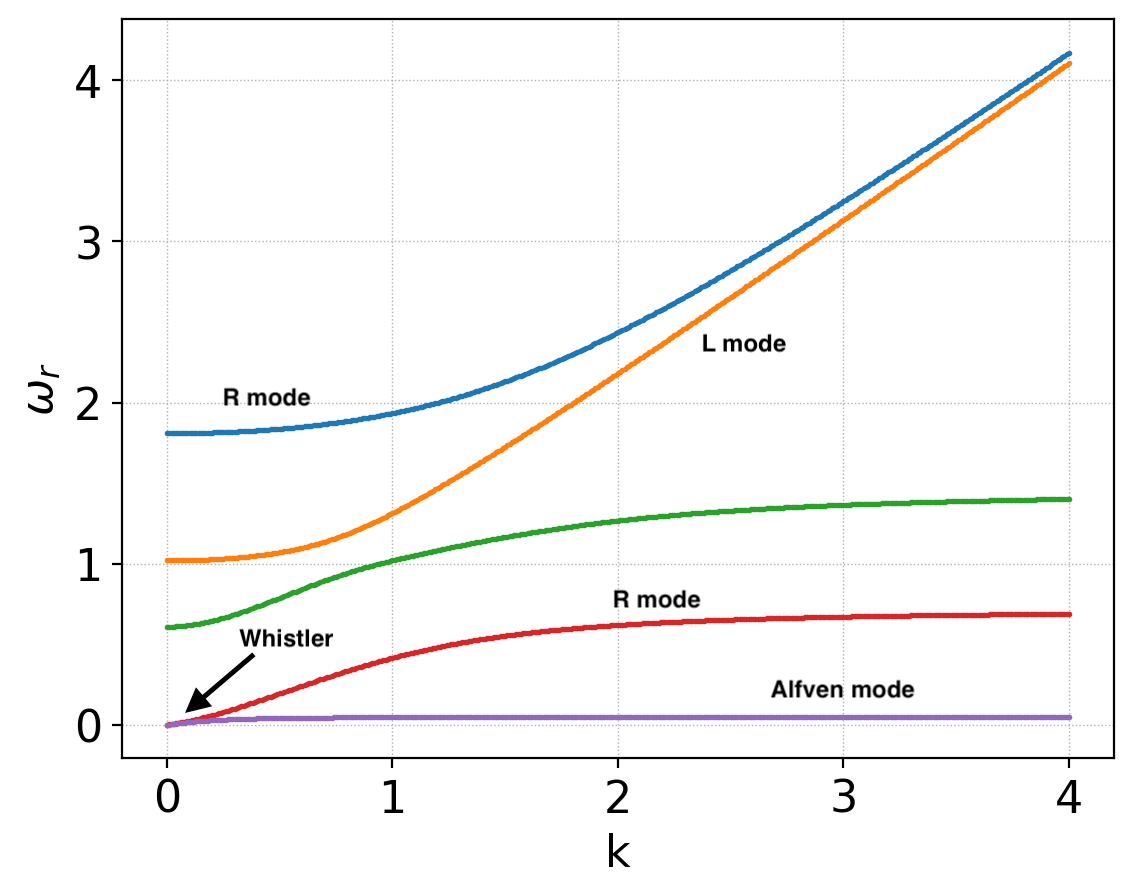
\includegraphics[width=\linewidth]{iso-cold-waves.png}
      \end{figure}
    \end{column}
  \end{columns}
  
\end{frame}

\begin{frame}{Essence of the finite-volume method}
  \small%
  Consider a PDE of the form (non necessarily hyperbolic)
  \begin{align*}
    \pfrac{\mvec{Q}}{t} + \pfrac{\mvec{F}}{x} = 0.    
  \end{align*}
  Now make a grid with cells $I_j = [x_{j-1},x_{j+1/2}]$ and
  $\Delta x = x_{j+1/2} - x_{j-1/2}$. The finite-volume method
  \emph{usually} evolves the cell-averages of the solution:
  \begin{align*}
    \pfrac{\mvec{Q}_j}{t} + \frac{\mvec{F}_{j+1/2} -\mvec{F}_{j-1/2} }{\Delta x} = 0
  \end{align*}
  where
  \begin{align*}
    \mvec{Q}_j(t) \equiv \frac{1}{\Delta x}\int_{I_j} \mvec{Q}(x,t) \thinspace dx
  \end{align*}
  are the \emph{cell-averages} and
  \begin{align*}
    \mvec{F}_{j\pm 1/2} \equiv \mvec{F}(\mvec{Q}_{j\pm 1/2})
  \end{align*}
  are \emph{numerical fluxes} at cell interfaces.

\end{frame}

\begin{frame}{Essence of the finite-volume method}
  \small%
  The finite-volume method \emph{usually} evolves the cell-averages of
  the solution:
  \begin{align*}
    \pfrac{\mvec{Q}_j}{t} + \frac{\mvec{F}_{j+1/2} -\mvec{F}_{j-1/2} }{\Delta x} = 0
  \end{align*}
  This equation is an \emph{exact} evolution equation for the
  cell-averages.\mypause%
  However, notice that
  \begin{itemize}
  \item We only know cell-averages $\mvec{Q}_{j}$ in each cell; we
    \emph{do not} know the \emph{cell-edge} values
    $\mvec{Q}_{j\pm 1/2}$ needed to compute the numerical flux
    $\mvec{F}_{j\pm 1/2}$.%
    \mypause%
  \item The finite-volume method consists of determining these
    \emph{edge values} and \emph{constructing a numerical-flux} so the
    cell-averages can be updated.
  \item Time-stepping can be done with a ODE solver (method-of-lines)
    or using a \emph{single-step} method (fully discrete scheme).
  \end{itemize}
  
\end{frame}

\begin{frame}{Essence of the finite-volume method}
\begin{columns}
  
  \begin{column}{0.5\linewidth}
    Instead of computing one edge value we will compute \emph{two}
    values: one the left and one on right of cell. With this, the
    numerical-flux will then be
    \begin{align*}
      \mvec{F}_{j+1/2} = \mvec{F}_{j+1/2}(\mvec{Q}^{-}_{j+1/2},\mvec{Q}^{+}_{j+1/2})
    \end{align*}
    We must impose the consistency condition:
    \begin{align*}
      \mvec{F}_{j+1/2}(\mvec{Q},\mvec{Q})
      = \mvec{F}(\mvec{Q}).
    \end{align*}
  \end{column}
  
  \begin{column}{0.5\linewidth}
    \begin{figure}    
    \setkeys{Gin}{width=1.0\linewidth,keepaspectratio}
    \incfig{FV-1D-grid.pdf}
  \end{figure}    
  \end{column}
\end{columns}  
\end{frame}

\begin{frame}{Cell-averages v/s cell-center values}
  \small%
  \begin{itemize}
  \item Typically, finite-volume schemes evolve the cell-average
    values; finite-difference schemes evolve cell-center (or nodal)
    values.%
    \mypause%
  \item For some low-order (first and some second-order) schemes the
    \emph{forms} of the scheme may look superficially the
    same. However, this is not true in general and one must \emph{very
      carefully} distinguish between cell-average and point-wise
    values. Otherwise incorrect schemes can result that ``look okay''
    but do not achieve full accuracy.%
    \mypause%
  \item What we evolve (cell-average, nodal values or in DG moments or
    interior node values) is called the \emph{solution
      representation}.
  \end{itemize}
  \begin{block}{Remember Your Representation}
    When studying or designing numerical schemes {\bf never} confuse
    one solution representation for another.
  \end{block}  
\end{frame}

\begin{frame}{Finite-Volume method computes \emph{mean} of flux gradient}
  To derive the basic form of the scheme we did
  \begin{align*}
    \frac{1}{\Delta x}\int_{I_j} \pfrac{F}{x} \thinspace dx =
    \frac{F_{j+1/2}-F_{j-1/2}}{\Delta x}.
  \end{align*}
  \begin{itemize}
  \item Notice that the left-hand side is the \emph{mean} of the flux
    gradient in the cell $I_j$
  \item Hence, in effect, the FV scheme is computing the \emph{mean}
    of the flux gradient and not the flux gradient itself. This is
    then used to update \emph{cell-average} of the solution.
  \item This is important to remember when computing source terms;
    making plots or computing diagnostics. (Remember Your
    Representation!).
  \end{itemize}
  
\end{frame}

\begin{frame}{Example: How to compute mean of \emph{product} of
    values?}
  \begin{itemize}
  \item Given cell-average values $Q_j$ and $V_j$ how can you compute
    cell-average value $(QV)_j$?%
    \mypause%
  \item Clearly, $(Q V)_j$ is not the same as $Q_j V_j$.%
    \mypause%
  \item In general, depending on the order of the scheme one has to
    \emph{recover} $Q(x)$ and $V(x)$ to sufficiently high order in a
    cell, multiply them and then compute the average of the
    product. Potential complications when solutions are not smooth
    enough.
  \item Almost never done! However, it may be important when trying to
    extract delicate information from simulations like turbulence
    spectra etc.
  \end{itemize}
\end{frame}

\begin{frame}{Essence of the finite-volume method}
  \footnotesize
  \begin{columns}
  
    \begin{column}{0.5\linewidth}
      Instead of computing one edge value we will compute \emph{two}
      values: one the left and one on right of cell-edge. We will next
      define a \emph{numerical flux function}
      \begin{align*}
        \mvec{G} = \mvec{G}(\mvec{Q}^{-}_{j+1/2},\mvec{Q}^{+}_{j+1/2})
      \end{align*}
      with \emph{consistency} condition
      \begin{align*}
        \lim_{\mvec{Q}_{L,R}\rightarrow Q} \mvec{G}(\mvec{Q}_L,\mvec{Q}_R) = \mvec{F}(\mvec{Q})
      \end{align*}
    \end{column}
  
    \begin{column}{0.5\linewidth}
      \begin{figure}    
        \setkeys{Gin}{width=0.7\linewidth,keepaspectratio}
        \incfig{FV-1D-grid.pdf}
      \end{figure}    
    \end{column}
  \end{columns}
  \mypause%
  In terms of the numerical flux function the FV update formula
  becomes
  \begin{align*}
    \pfrac{\mvec{Q}_j}{t} + \frac{\mvec{G}(\mvec{Q}_{j+1/2}^+,\mvec{Q}_{j+1/2}^-) - \mvec{G}(\mvec{Q}_{j-1/2}^+,\mvec{Q}_{j-1/2}^-)}{\Delta x} = 0    
  \end{align*}
\end{frame}

\begin{frame}{Steps in constructing finite-volume method}
  \begin{align*}
    \pfrac{\mvec{Q}_j}{t} + \frac{\mvec{G}(\mvec{Q}_{j+1/2}^+,\mvec{Q}_{j+1/2}^-) - \mvec{G}(\mvec{Q}_{j-1/2}^+,\mvec{Q}_{j-1/2}^-)}{\Delta x} = 0    
  \end{align*}
  Hence, to completely specify a finite-volume scheme we must design
  algorithms for each of the following three steps:
  \begin{itemize}\cramplist
  \item {\bf Step 1}: A {\bf recovery scheme} (possibly with limiters)
    to compute the left/right interface values $\mvec{Q}^{\pm}$ at
    each interface using a set of cell-average values around that
    interface,%
    \mypause%
  \item {\bf Step 2}: A {\bf numerical flux function} that takes the
    left/right values and returns a consistent approximation to the
    physical flux, and%
    \mypause%
  \item {\bf Step 3}: A {\bf time-stepping scheme} to advance the
    solution in time and compute the cell-averages at the next
    time-step.
  \end{itemize}
\end{frame}

\begin{frame}{Some notation for use in recovery stencils}
  \footnotesize%
  Example: symmetric recovery across two cells can be written as
  \begin{align*}
    Q_{i+1/2} = \frac{1}{2}(Q_{i+1}+Q_j) = \frac{1}{2}(d_p + d_m) Q_{i+1/2}
  \end{align*}
  Example: central difference scheme for second derivative:
  \begin{align*}
    \frac{\partial^2 Q_i}{\partial x^2}
    = \frac{1}{\Delta x^2} (Q_{i+1} - 2 Q_j + Q_{i-1})
    = \frac{1}{\Delta x^2} (\Delta_p - 2I + \Delta_m) Q_i
  \end{align*}      
  \begin{figure}
    \setkeys{Gin}{width=0.75\linewidth,keepaspectratio}
    \incfig{stencil-ops.png}
    \caption{Basic indexing operators to move from cell to cell, face
      to cell and cell to face.}
  \end{figure}
\end{frame}

\begin{frame}{Recovery scheme: four-cell stencil, centered scheme}
  \footnotesize%
  \begin{figure}
    \setkeys{Gin}{width=0.35\linewidth,keepaspectratio}
    \incfig{4c-stencil.png}
  \end{figure}  
  \begin{itemize}
  \item To construct a four-cell symmetric stencil recovery across an
    interface we will use a four-cell stencil:
    $\{d_{2m}, d_m, d_p, d_{2p} \}$%
    \mypause%
  \item Setup a local coordinate system with $x=0$ at the interface
    and assume a polynomial recovery
    \begin{align*}
      p(x) = p_0 + p_1 x + p_2 x^2 + p_3 x^3
    \end{align*}
    \mypause%
  \item Match the cell-averages of $p(x)$ in each of the cells
    $\{d_{2m}, d_m, d_p, d_{2p} \}$ to get a system of linear
    equations. Solve this system to determine $p_0, p_1, p_2, p_3$.
  \end{itemize}
\end{frame}

\begin{frame}{Recovery scheme: four-cell stencil, centered scheme}
  Solving the system of four equations for the four coefficients
  $p_i$, $i=0,\ldots,3$ yields:
  \begin{align*}
    p_0 &=  \frac{1}{12}(-d_{2m} + 7 d_m + 7 d_p - d_{2p}) Q \\
    p_1 &=  \frac{1}{12\Delta x}(d_{2m} - 15 d_m + 15 d_p - d_{2p}) Q \\
    p_2 &=  \frac{1}{4 \Delta x^2}(d_{2m} - d_m - d_p + d_{2p}) Q \\
    p_4 &=  \frac{1}{6 \Delta x^3}(d_{2m} - 3d_m + 3 d_p - d_{2p}) Q.
  \end{align*}
  \begin{itemize}
  \item Notice: stencils of the even coefficients are \emph{symmetric}
    and the odd coefficients are \emph{anti-symmetric}.%
    \mypause%
  \item To compute the interface value we do not really need all of
    these coefficients but only need to evaluate the recovery
    polynomial at $x=0$, i.e we only need $p(0) = p_0$
  \end{itemize}
\end{frame}

\begin{frame}{Recovery scheme: four-cell stencil, centered scheme}
  \small%
  To compute the interface value we do not really need all of these
  coefficients but only need to evaluate the recovery polynomial at
  $x=0$, i.e we only need $p(0) = p_0$. Hence, the interface value can
  be computed from
  \begin{align*}
    Q^+ = Q^- = \frac{1}{12}(-d_{2m} + 7 d_m + 7 d_p - d_{2p}) Q.
  \end{align*}
  Note that due the symmetric nature of the stencil we have only a
  \emph{single} value at the interface. This means that the numerical
  flux function at an interface is simply
  \begin{align*}
    G(Q,Q) = F(Q)
  \end{align*}
  from consistency requirements.%
  \mypause%
  This completes the spatial finite-volume discretization! The scheme
  one gets from this is very accurate (even ``structure preserving''
  for Maxwell equations), though not very robust in presence of sharp
  gradients. (No Free Lunch)
\end{frame}

\begin{frame}{How accurate is any given scheme?}
  To fix ideas consider we wish to solve the advection equation
  \begin{align*}
    \pfrac{f}{t} + \pfrac{f}{x} = 0
  \end{align*}
  Using the four-cell symmetric recovery scheme to compute interface
  values in the FV update formula we get the semi-discrete scheme
  \emph{five-cell stencil} update formula:
  \begin{align*}
    \pfrac{f_j}{t}
    = -\frac{1}{\Delta x}\int_{x_{j-1/2}}^{x_{j+1//2}}
    \pfrac{f}{x} \thinspace dx
    =
    -\frac{1}{12 \Delta x} (f_{j-2} - 8f_{j-1} + 8 f_{j+1} - f_{j+2})
  \end{align*}
  How accurate is this scheme, or what is its order of convergence?
\end{frame}

\begin{frame}{How accurate is any given scheme? Use Taylor series}
  \footnotesize%
  \begin{itemize}\cramplist
  \item Take a Taylor series polynomial around the cell center of cell
    $I_j = [-\Delta x/2, \Delta x/2]$ locally at $x=0$
    \begin{align*}
      T(x) = \sum_{n=0} \frac{T_n}{n!} x^n.
    \end{align*}
    \mypause%
  \item Compute the cell average of this polynomial in each of the
    stencil cells $\{\Delta_{2m}, \Delta_m, \Delta_p, \Delta_{2p} \}$
    \mypause%
  \item Substitute these averages in the update formula to compute the
    mean value of the flux gradient in the cell
    $I_j = [-\Delta x/2, \Delta x/2]$
    \begin{align*}
      \frac{1}{12 \Delta x} (\Delta_{2m} - 8\Delta_m + 8 \Delta_p -
      \Delta_{2p}) T
      =
      T_1 + \frac{\Delta x^2}{24} T_3  - \frac{21 \Delta x^4}{640} T_5 + \ldots
    \end{align*}
    \mypause%
  \item Subtract the exact cell average of the gradient of the Taylor
    polynomial in cell $I_j = [-\Delta x/2, \Delta x/2]$, i.e.
    \begin{align*}
      \frac{1}{\Delta x}\int_{-\Delta x/2}^{\Delta x/2} \pfrac{T}{x} \thinspace dx
      =
      T_1 + \frac{\Delta x^2}{24} T_3  + \frac{\Delta x^4}{1920} T_5 + \ldots
    \end{align*}
    from the stencil computed value. The remainder term is the error
    of the scheme.
  \end{itemize}  
\end{frame}

\begin{frame}{Symmetric four-cell recovery scheme is fourth-order
    accurate}
  The above procedure (needs use of a compute algebra system to
  simplify the computations) shows that the symmetric four-cell
  recovery scheme has error that goes like
  \begin{align*}
      \frac{\Delta x^4}{30} T_5 + O(\Delta x^6)
  \end{align*}
  showing the scheme converges with \emph{fourth-order} accuracy
  $O(\Delta x^4)$ for linear advection equation. (Reducing $\Delta x$
  by 2 reduces error by a factor of $16$).

\end{frame}

\begin{frame}{Accuracy is not everything: dispersion and diffusion}
  \footnotesize
  \begin{itemize}
  \item High-order symmetric schemes like the one we derived are very
    accurate (even ``structure preserving'' for some problems) but not
    robust.
    \mypause%
  \item Two other properties of the scheme are important to
    understand: \emph{dispersion} and \emph{diffusion}. For this we
    wil derive a \emph{numerical dispersion relation} analogous to
    dispersion relation we derived for linearized systems.
    \mypause%
  \item Consider a single mode $f(x) = e^{ik x}$ where $k$ is the
    wavenumber. Compute the cell-average of the mode on each of the
    cells in the stencil, plug into the stencil formula to derive the
    \emph{numerical dispersion relation}
    \begin{align*}
      i\overline{k} = \sum_{m=-N}^{M} c_m e^{i k m \Delta x}
    \end{align*}
    where we have written the stencil in the generic form
    \begin{align*}
      \frac{1}{\Delta x}\sum_{m = -N}^{M} c_m f_{j+m}
    \end{align*}

  \end{itemize}
\end{frame}

\begin{frame}{Symmetric four-cell recovery scheme has no diffusion!}
  \small
  \begin{columns}
    
    \begin{column}{0.6\linewidth}
      \begin{itemize}
      \item Note that the numerical dispersion relation will in
        general give a \emph{complex} effective wavenumber
        $\overline{k}$.
      \item The dispersion relation for a hyperbolic equation is
        $\omega = \lambda k$. Hence, the \emph{real part} of
        $\overline{k}$ represents dispersion and \emph{imaginary part}
        of $\overline{k}$ represents diffusion/growth. Obviously, we
        want imaginary part to be \emph{negative} to avoid solution
        blow-up!
      \item The four-cell symmetric stencil has \emph{no imaginary
          part} of $\overline{k}$. This related to the fact that it is
        \emph{symmetric} (anti-symmetric stencil coefficients). This
        is not necessarily a good thing!
      \end{itemize}
    \end{column}
  
    \begin{column}{0.4\linewidth}
      \begin{figure}
        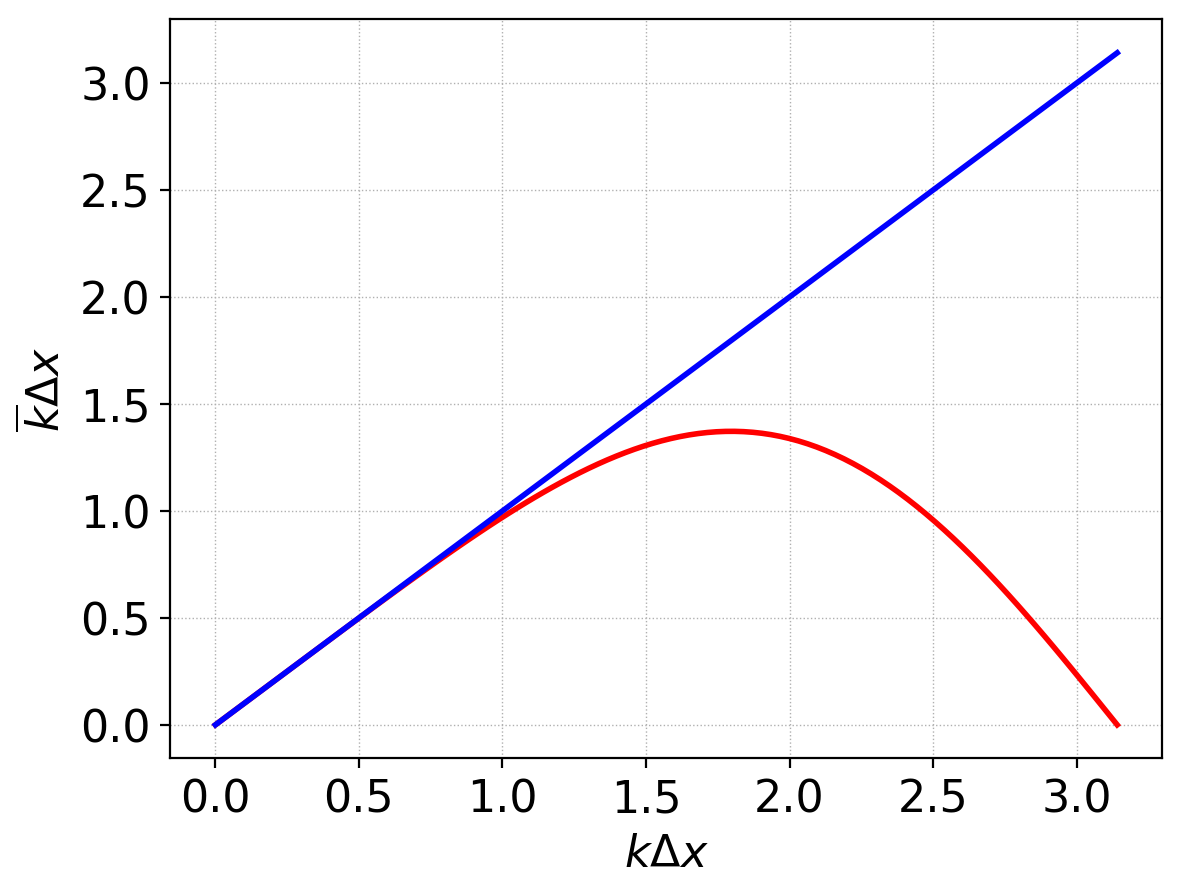
\includegraphics[width=\linewidth]{5p-kbar.png}
        \caption{Real-part of numerical dispersion relation for
          four-cell recovery scheme. Notice the strong dispersion for
          higher-$k$ modes}
      \end{figure}
    \end{column}
  \end{columns}

\end{frame}

\begin{frame}{Numerical Flux Function}
  \footnotesize%
  The numerical flux function computes a \emph{consistent} flux at the
  cell-edge from the cell averages.
  \begin{align*}
    \lim_{\mvec{Q}_{L,R}\rightarrow Q} \mvec{G}(\mvec{Q}_L,\mvec{Q}_R) = \mvec{F}(\mvec{Q}).
  \end{align*}
  Examples
  \begin{itemize}
  \item \emph{Central Flux} in which we simply average the flux from
    the two states at the interface
    \begin{align*}
      \mvec{G}(\mvec{Q}_L,\mvec{Q}_R) = \frac{1}{2}
      \left( \mvec{F}(\mvec{Q}_L) + \mvec{F}(\mvec{Q}_R) \right) .
    \end{align*}
  \item \emph{Upwind Flux} in which we choose the edge on the
    ``upwind'' side to account for direction of information flow:
    \begin{align*}
      \mvec{G}(\mvec{Q}_L,\mvec{Q}_R) = \mvec{F}(\mvec{Q}_L)
    \end{align*}
    if information is flowing from left-to-right, and
    \begin{align*}
      \mvec{G}(\mvec{Q}_L,\mvec{Q}_R) = \mvec{F}(\mvec{Q}_R)
    \end{align*}
    if information is flowing from right-to-left. Begs the question:
    how to determine which direction information is flowing in?
    Answer: the eigensystem of the hyperbolic equation contains this!
  \end{itemize} 
\end{frame}

\begin{frame}{Numerical Flux Function: Lax flux}
  \small%
  \begin{itemize}
  \item A good choice of the numerical flux function is the
    \emph{local Lax} flux:
    \begin{align*}
      \mvec{G}(\mvec{Q}_L,\mvec{Q}_R) = \frac{1}{2}
      \left( \mvec{F}(\mvec{Q}_L) + \mvec{F}(\mvec{Q}_R) \right)
      - \frac{|\lambda|}{2}( \mvec{Q}_R - \mvec{Q}_L )
    \end{align*}
    where $|\lambda|$ is an estimate of the (absolute) maximum of all
    eigenvalues at the interface.%
    \mypause%
  \item   For advection equation this becomes
    \begin{align*}
      G(f_L,f_R) = \frac{1}{2} a ( f_L + f_R ) - \frac{|a|}{2}( f_R - f_L )
    \end{align*}
    This works for either sign of advection speed $a$, automatically
    giving upwinding.%
    \mypause%
  \item Note $|\lambda|$ is only a local (to the interface)
    \emph{estimate}. You can use a global estimate too: orginal
    formulation by Peter Lax (``Lax fluxes'').
  \end{itemize}

\end{frame}

\begin{frame}{Numerical Flux Function: Systems of equations}
  \small%
  \begin{itemize}
  \item Lax flux is a good ``first'' flux to use. However, notice it
    only takes into account a \emph{single} piece of information:
    maximum eigenvalue.%
    \mypause%
  \item For a \emph{linear system} of equations (Maxwell equation) or
    \emph{locally linearized} nonlinear system we can instead do
    \begin{align*}
      G(Q_R,Q_L) = \frac{1}{2}\big(F(Q_R)+F(Q_L)\big) - \frac{1}{2}(A^+\Delta Q_{R,L} - A^-\Delta Q_{R,L})      
    \end{align*}
    where the \emph{fluctuations} $A^\pm\Delta Q$ are defined as
    \begin{align*}
      A^\pm\Delta Q_{R,L} \equiv \sum_p r^p \lambda^\pm_p (w_R^p-w_L^p) = \sum_p r^p \lambda^\pm_p l^p(Q_R-Q_L).
    \end{align*}
    where $\lambda_p^+ = \max(\lambda_p,0)$ and
    $\lambda_p^- = \min(\lambda_p,0)$.%
    \mypause%
  \item Additional care is needed for nonlinear equations like Euler
    or ideal MHD equations. More on this on Thursday.
  \end{itemize}
\end{frame}

\begin{frame}{Godunov's Theorem}
  \small%
  \begin{itemize}
  \item A very important theorem proved by Godunov is that there is {
      \bf no} \emph{linear scheme} that is ``monotonicity preserving''
    (no new maxima/minima created) and {\bf higher than first-order
      accurate}!  \mypause%
  \item Consider a general scheme for advection equation
    \begin{align*}
      f_j^{n+1} = \sum_k c_k f_{j+k}^n.
    \end{align*}
    The discrete slope then is
    \begin{align*}
      f_{j+1}^{n+1} - f_j^{n+1} = \sum_k c_k \left( f_{j+k+1}^n - f_{j+k}^n \right).
    \end{align*}
    Assume that all $f_{j+1}^n - f_j^n > 0$. To maintain monotonicity
    at next time-step hence one must have all $c_k \ge 0$.
  \end{itemize}
\end{frame}

\begin{frame}{Godunov's Theorem}
  \small%
  \begin{itemize}
  \item First order upwind scheme:
    \begin{align*}
      f_j^{n+1} = f_j^n -\frac{\Delta t}{\Delta x}(f_j^n - f_{j-1}^n)
    \end{align*}
    this satisfies monotonicity as long as
    ${\Delta t}/{\Delta x} \le 1$.%
    \mypause%
  \item Second order symmetric scheme
    \begin{align*}
      f_j^{n+1} = f_j^n -\frac{\Delta t}{2 \Delta x}(f_{j+1}^n - f_{j-1}^n)
    \end{align*}
    clearly this does not satisfy the condition of monotonicity.
    \mypause%
  \item In general condition on Taylor series to ensure atleast
    second-order accuracy shows that at least \emph{one} of the $c_k$s
    must be negative. Hence, by contradiction, \emph{no such scheme
      exists}!
  \end{itemize}
\end{frame}

\begin{frame}{Godunov's Theorem: Unfortunate Consequences and Workarounds}
  \small%
  \begin{itemize}
  \item Godunov's Theorem is highly distressing: accurate
    discretization seems to preclude a scheme free from monotonicity
    violations
    \mypause%
  \item One way around is to start with a linear scheme that is very
    accurate and then add some local diffusion to it to control the
    monotonicity.%
    \mypause%
  \item However, Godunov's theorem shows that this ``diffusion'' must
    be dependent on the local solution itself and can't be fixed
    \emph{a priori}. This means a {\bf monotonicity preserving scheme
      must be nonlinear}, even for linear hyperbolic equations.%
    \mypause%
  \item Leads to the concept of \emph{nonlinear limiters} that control
    the monotonicity violations (adding diffusion to high-$k$ modes).
    No free lunch: limiters must diffuse high-$k$ modes but this will
    inevitably lead to issues like inability to capture, for example,
    high-$k$ turbulence spectra correctly without huge grids.
  \item Major research project: interaction of shocks, boundary layers
    and turbulence in high-Reynolds number flows.
  \end{itemize}
\end{frame}

\begin{frame}{Nonlinear flux limiters: Getting around Godunov's Theorem}
  \small%
  To get around Godunov's Theorem we need to construct a
  \emph{nonlinear scheme}, even for linear equations. One apporach is
  to use nonlinear flux-limiters:
  \begin{align*}
    \mvec{F}_{j+1/2} = \phi(r_{j+1}) \mvec{F}^H_{j+1/2} + \big(1-\phi(r_{j+1})\big) \mvec{F}^L_{j+1/2}
  \end{align*}
  where $\phi(r)>0$ is a \emph{limiter} function: chooses between
  \emph{high-order} and \emph{low-order} flux.
  \mypause%
  \begin{itemize} 
  \item What are the low- and high-order fluxes? For high-order
    fluxes: use either symmetric or higher-order upwind-biased
    recovery to construct the flux. For low-order use first-order
    upwind fluxes.
  \end{itemize}
  \mypause%
  The first-order upwind flux is ``Total-Variation Diminishing''
  (TVD), $\textrm{TV}(f^{n+1}) \le \textrm{TV}(f^n)$ where
  ``Total-Variation'' is defined as:
  \begin{align*}
    \textrm{TV}(f) = \sum_j | f_{j+1} - f_{j} |
  \end{align*}
\end{frame}

\begin{frame}{Nonlinear flux limiters}
  \small
  \begin{columns}
    \begin{column}{0.5\linewidth}
      The limiter function $\phi(r)$ depends on an estimate of the
      \emph{relative} slopes at an interface. For example, one choice
      is
      \begin{align*}
        r_{j+1/2} = \frac{\textrm{\textrm{slope at upwind-edge}}}{\textrm{slope at } j+1/2}
      \end{align*}
      (For systems of equations one needs limit each eigenvector
      instead). With this, choose a function that maintains TVD
      property. Eg, min-mod limiter
      \begin{align*}
        \phi(r) = \max\big(0, \min(2r, (1+r)/2,2) \big).
      \end{align*}
    \end{column}
    
    \begin{column}{0.5\linewidth}
      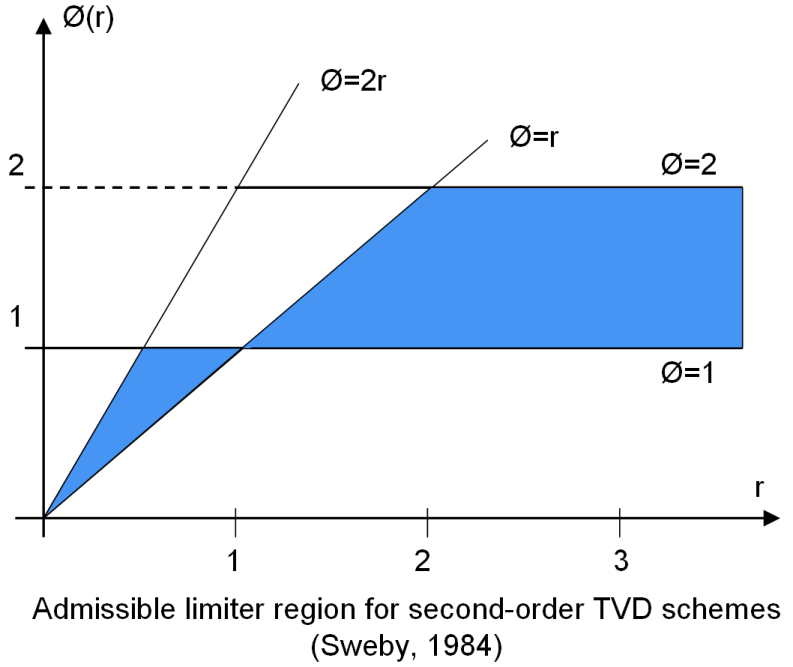
\includegraphics[width=\linewidth]{LimiterRegion.png}
    \end{column}
  \end{columns}
  See Wikipedia page
  \url{https://en.wikipedia.org/wiki/Flux_limiter}. (Not very
  high-quality but gives you a general idea).
\end{frame}

\begin{frame}{Nonlinear flux limiters: No ``Perfect'' Limiter!}
  \small
  \begin{columns}
    \begin{column}{0.5\linewidth}
      \begin{itemize}
      \item Unfortunately, there is no perfect limiter (though some
        come close to perfection): depends on problem and best to
        implement many!
      \item Most limiters ``chop off'' genuine maxima/minima: notice
        that $\phi(r<0) = 0$ which means that if there is a genuine
        maxima/minima then low-order flux is selected.
      \item Tricky to distinguish step-function from parabola!
        ``Best'' limiter (IMO): Suresh and Huynh, JCP {\bf 136}, 83-99
        (1997). Not an easy paper to understand.
      \end{itemize}
    \end{column}
    
    \begin{column}{0.5\linewidth}
      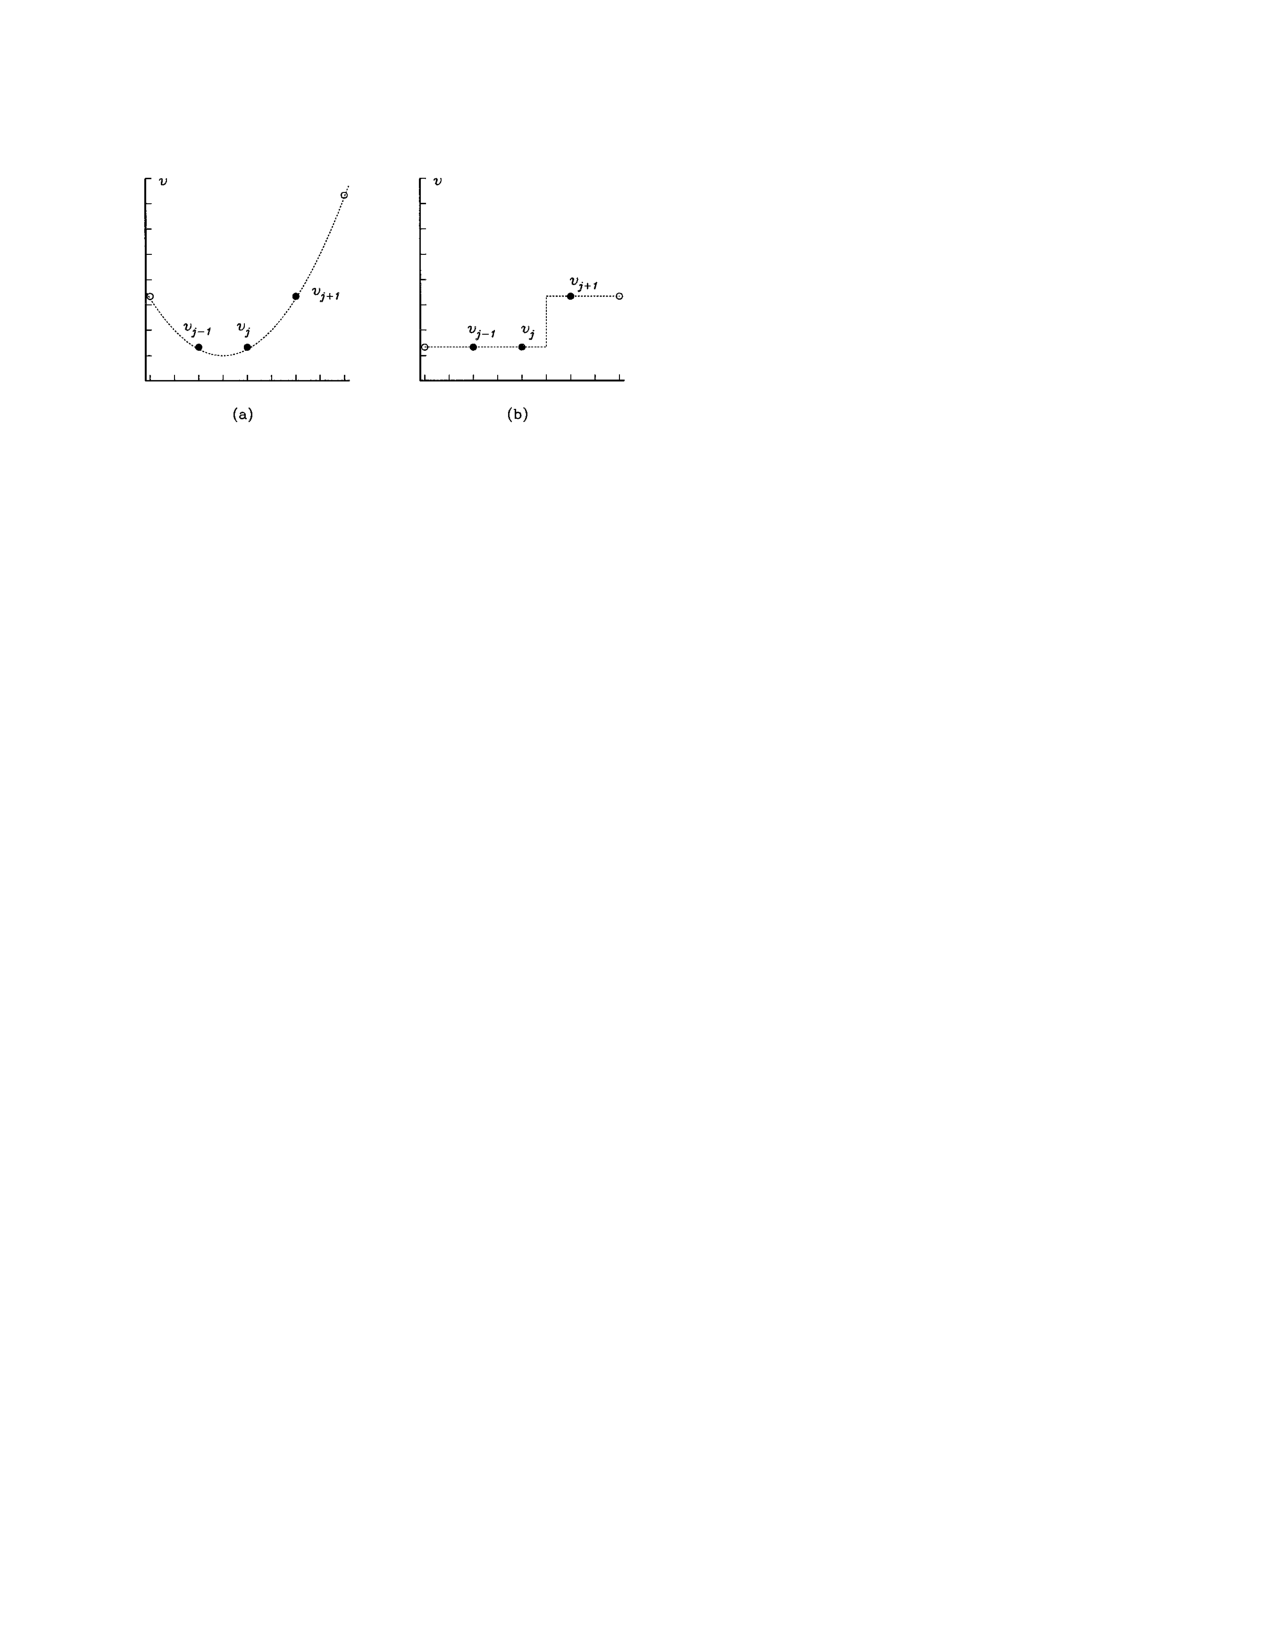
\includegraphics[width=\linewidth]{suresh-huynh.pdf}
    \end{column}
  \end{columns}
\end{frame}

\begin{frame}{Some Parting Thoughts and All the Best!}
  \small
  Here are some personal parting thoughts on computational physics:
  \begin{itemize}
  \item Computational physics is a rapidly evolving field. Good field
    to be in!
  \item Strive for {\bf technical excellence}. Do not settle for
    existing methods or tools and spend time in understanding deeply
    {\bf both} the physics of the equations \emph{and} the numerics
    used to solve them. Go beyond your classwork and thesis reasearch
    (make it a point to read arxiv physics.comp-ph and math.NA
    postings \emph{every day}).
  \item Modern computational physics is moving to C and C++: please
    learn them. Use good software practices (write modular code, use
    version control, build systems, regression tests). Even for your
    thesis code!
  \item To become \emph{really good} you must {\bf apprentice
      yourself} to a genuine expert.
  \item If you become an expert at the (i) physics (ii) mathematics of
    the numerical methods (iii) programming and software techniques,
    you will be in a very strong position to contribute to development
    in many different fields. You will bring \emph{unique skills}
    which few other people will be able to match.
  \end{itemize}
\end{frame}

\end{document}


\begin{frame}{}
\end{frame}

\begin{columns}
  
  \begin{column}{0.6\linewidth}
  \end{column}
  
  \begin{column}{0.4\linewidth}
    \includegraphics[width=\linewidth]{fig/Kinsey_2011_Pfus_vs_T.pdf}
  \end{column}
\end{columns}

% ----------------------------------------------------------------
